\chapter{Descrição do problema}\label{cap:descprob}

Com um conjunto de voos atribuído a uma mesma frota tem-se a necessidade de
sequência-los de forma que cada aeronave possa ficar responsável por uma
sequência válidas de voos que são chamada de trilho. Um conjunto de voos está
bem sequenciado se é possível atende-los com o menor número de aeronáves e com a
menor alteração do planejamento inicial desses voos.
 
Esse problema apresenta uma grande quantidade de restrições que devem ser
atendidas. Essas restrições foram obtidas a partir da literatura e também da
legislação vigente. Ainda podem existir outras restrições, porém
atualmente existe uma lacuna causada pela falta de comunicação entre a
academia e as empresas que, em sua grande maioria, são fechadas a esse tipo de
comunicação com a finalidade de proteger seus ativos.

As principais restrições que envolvem o PCTA são as temporais e as geográficas.
Essas duas restrições são triviais e representam respectivamente que uma voo não
pode partir antes da chegada de seu antecessor e que um voo não pode partir de
um local diferente do voo que lhe antecede, a não ser que haja tempo para a
criação de um voo de reposicionamento. 

Deve-se levar em consideração também o
tempo de solo que representa o tempo que o avião tem que permanecer no solo a
cada pouso. Esse tempo é requerido para efetuar o reabastecimento da aeronave e a
troca de passageiros que chegaram ao seu destino ou que irão fazer conexões no
aeroporto que a aeronave pousou. Esse tempo é variável dependendo do
aeroporto e do tipo da aeronave que está sendo operada. Adicionalmente esse
tempo pode ser acrescido se houver necessidade de efetuar a trocar da
tripulação.

Existe também a possibilidade de modificar o tempo de partida dos voos
planejados, no entanto essas mudanças são prejudiciais para a companhia, por
alterar o horário que foi inicialmente definido pela demanda, e por isso são
penalizadas se adicionadas a solução. Também é possível efetuar a ligação de
voos que estão em aeroportos diferentes a partir da criação de um voo de
reposicionamento, ou seja, de um voo que não estava no planejamento
inicial.

Essas restrições induzem a formação de uma rede de possíveis conexões entre
voos, essas conexões são denominadas de tipo de arco. Porém para conseguir
melhores resultados deve-se permitir uma maior flexibilidade na construção dos
trilhos permitindo mudanças no tempo de partida sugerido dos voos e
também a criação de voos de reposicionamento.

A ligação dos voos pode ocorrer de 6 formas distintas. Os arcos do tipo 1
permitem a ligação de voos sem a utilização de atrasos e/ou reposicionamento.
Os arcos do tipo 2 utilizam atrasos mas não o reposicionamento. Os arcos do
tipo 3 permitem o sequenciamento com a utilização de um voo de reposicionamento
mas sem inserir atraso em nenhum dos voos envolvidos. Os arcos do tipo 4
utilizam-se de atrasos e de um voo de reposicionamento para fazer a ligação
entre dois voos. Os arcos do tipo 5 e 6 são usados na modelagem matemática, que
foi formulado como um problema de minimização de fluxos em rede, para
representar respectivamente o nó origem(source) e o destino(sink). Abaixo um
maior detalhamento desses arcos:
  
\begin{itemize}
\item Conexão natural (Arco do tipo 1) - Os arcos desse tipo conectam dois voos
respeitando o tempo de partida sugerido e a restrição geográfica. Eles são
associados com as ligações que não requerem mudanças no tempo de partida e nem
precisam de voos de reposicionamento. O arco do tipo 1 não apresenta custo para
ser adicionado a solução.

\begin{figure}[ht]
	\caption{Representação esquemática do arco do tipo 1. \mbox{Fonte: (Própria)}}
	\label{fig:arc1}
	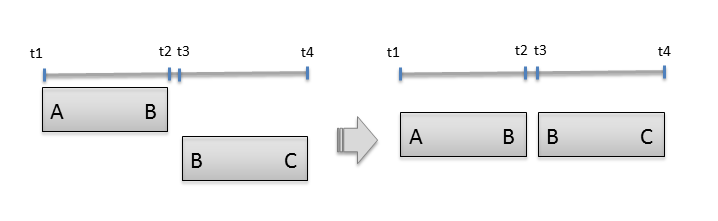
\includegraphics[scale=0.35]{./img/arc1}
	
\end{figure}

\item Mudança no tempo (Arco do tipo 2) - Apesar de ter os voos incidentes no
mesmo aeroporto, os arcos desse tipo não permitem a ligação de forma direta
pois o tempo de solo disponível não é suficiente para permitir a ligação. No
entanto, a escolha desse tipo de arco implica em uma mudança no tempo de
partida sugerido para quaisquer um dos voos envolvidos. O custo de um arco
desse tipo é igual a soma dos valores absolutos dos atrasos (em minutos) dos
horários de partida envolvidos.
      
\begin{figure}[ht]
	\caption{Representação esquemática do arco do tipo 2. \mbox{Fonte: (Própria)}}
	\label{fig:arc2}
	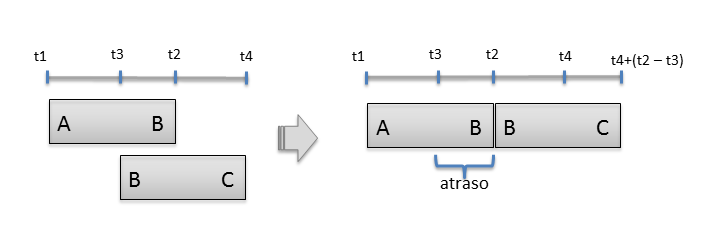
\includegraphics[scale=0.35]{./img/arc2}
	
\end{figure}

\item Voos de reposicionamento (Arco do tipo 3) - Esses arcos representam
conexões entre dois voos em que a origem parte de um aeroporto diferente do
local de partida do voo de destino, no entanto, existe tempo suficiente para um
voo de reposicionamento, entre os dois locais, sem violar as restrições de
tempo de solo. Os custos de um arco do tipo 3 é igual a duração do voo de
reposicionamento, incluindo o seu tempo de solo.

\begin{figure}[ht]
	\caption{Representação esquemática do arco do tipo 3. \mbox{Fonte: (Própria)}}
	\label{fig:arc3}
	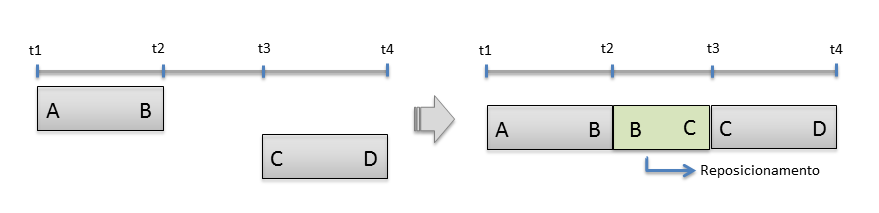
\includegraphics[scale=0.35]{./img/arc3}
	
\end{figure}

\item Voos de reposicionamento mais mudança de tempo (Arco do tipo 4) - Esses
arcos representam conexões que precisam de um voo de reposicionamento mais
mudança no tempo de partida sugerido. O arco do tipo 4 tem custo igual tempo do
voo de reposicionamento, incluindo o tempo de solo, mais a soma dos atrasos dos
horários de partida envolvidos em valor absoluto.

\begin{figure}[ht]
	\caption{Representação esquemática do arco do tipo 4. \mbox{Fonte: (Própria)}}
	\label{fig:arc4}
	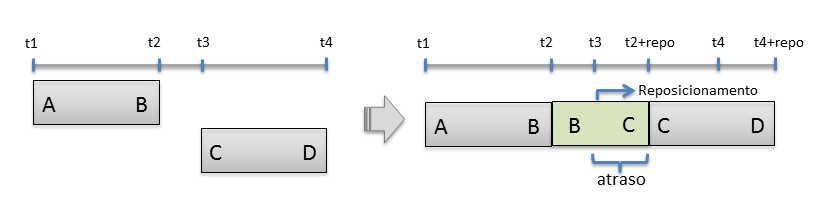
\includegraphics[scale=0.35]{./img/arc4}
	
\end{figure}

\item Arcos do nó fonte ou \textit{source} (Arco do tipo 5) - Esses, arcos são
criados para identificar o inicio de um trilho e é com ele também que se sabe a
quantidade de trilhos necessários para resolver o problema. Cada arco do tipo 5
tem o custo igual a 1000.

\item Arcos do nó final ou \textit{sink} (Arco do tipo 6) - Esses arcos tem
como destino o nó fictício que é usado para finalizar um trilho no modelo. Os
arcos do tipo 6 não tem custo.

\end{itemize}

Abaixo na Figura \ref{fig:arpexample} temos um exemplo visual de como a forma
que é feita a montagem dos trilhos das aeronaves podem influênciar de forma
significativa na utilização dos recursos da companhia aérea. Cada
retangulo representa um voo onde a parte laranja representa o tempo de solo que
cada voo deve obedecer e a azul o tempo de voo esperado da cidade de origem para
a cidade de destino. As letras representam aeroportos diferentes e a linha
pontilhada indica o tempo de inicio e de termino de cada voo, ela é importante
para identificação dos atrasos.

\begin{figure}[ht]
	\caption{Construção de Trilhos de Aeronaves. \mbox{Fonte: (Própria)}}
	\label{fig:arpexample}
	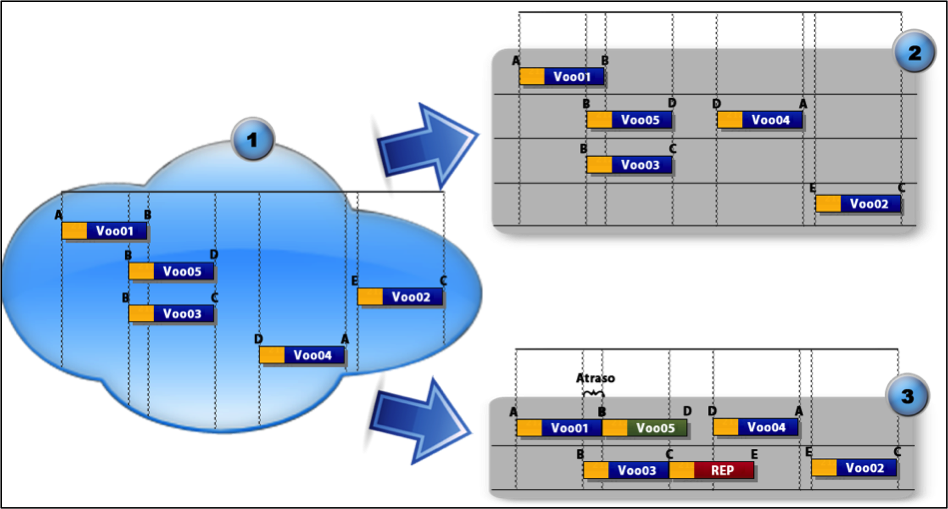
\includegraphics[scale=0.6]{./img/arpexample}
	
\end{figure}

A parte 1 da Figura \ref{fig:arpexample} representa os voos da companhia que
ainda não foram cobertos por nenhuma aeronave e nas partes 2 e 3 são
demonstrado duas formas de organizar esses voos em trilhos.

Na parte 2 temos a melhor forma possível de se organizar os voos disponíveis
utilizando apenas os arcos do tipo 1, ou seja sem a utilização de atrasos ou de
voos de reposicionamento. Dessa forma se consegue uma formação com 4 trilhos.

Na parte 3 temos a melhor forma de organizar os voos com a possibilidade de
utilizar qualquer tipo de ligação e com um atraso máximo igual a um tempo de
solo. Pode-se verificar que atrasando um voo e criando outro de
reposicionamento consegue-se economizar duas aeronaves, gerando uma solução com
apenas 4 trilhos.

Pode-se verificar que a utilização de diferentes tipos de arcos pode
proporcionar uma melhora significativa na qualidade da solução. Porém essa
abordagem faz com que a complexidade e a quantidade das soluções
cresça muito e por isso a escolha dos tipos de ligações entre os voos
deve ser feita de forma cuidadosa.

%%MOSTRAR A MALHA DA GOL/TAM/DELTA ?